\documentclass{standalone}
\usepackage{ tikz }
\usepackage{ xparse }
\input{macros/all}

\begin{document}
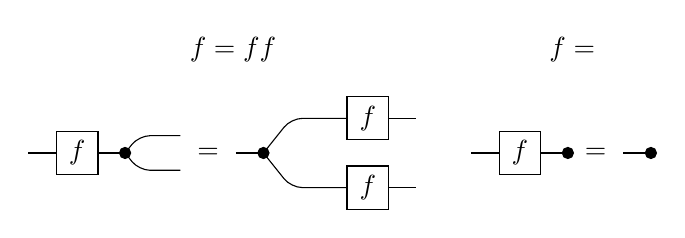
\begin{tikzpicture}[yscale=-1,x=1em,y=1.25em]

    \draw (0.5,0) -- (1.5,0);
    \node[draw, minimum height = 1.5em, minimum width = 1.5em, anchor = west] at (1.5,0){$f$};
    \draw (3,0) -- (4,0);
    \filldraw (4,0) circle (2pt);
    \draw [rounded corners] (4,0) -- (4.5,-0.5) -- (6,-0.5);
    \draw [rounded corners] (4,0) -- (4.5,0.5) -- (6,0.5);

    \node at (7,0) {$=$};
    \node at (7.9,-3) {$f \seq \ccopy{} = \ccopy{} \seq f \tensor f$};

    \draw (8,0) -- (9,0);
    \filldraw (9,0) circle (2pt);
    \draw [rounded corners] (9,0) -- (10,-1) -- (12,-1);
    \draw [rounded corners] (9,0) -- (10,1) -- (12,1);

    \node[draw, minimum height = 1.5em, minimum width = 1.5em, anchor = west] at (12,-1){$f$};
    \node[draw, minimum height = 1.5em, minimum width = 1.5em, anchor = west] at (12,1){$f$};

    \draw (13.5,-1) -- (14.5,-1);
    \draw (13.5,1) -- (14.5,1);

    \draw (16.5, 0) -- (17.5,0);
    \node[draw, minimum height = 1.5em, minimum width = 1.5em, anchor = west] at (17.5,0){$f$};
    \draw (19,0) -- (20,0);
    \filldraw (20,0) circle (2pt);

    \node at (20.3,-3) {$f \seq \cdel{} = \cdel{}$};
    \node at (21,0) {$=$};

    \draw (22,0) -- (23,0);
    \filldraw (23,0) circle (2pt);

\end{tikzpicture}
\end{document}